\documentclass[12pt]{report}
\usepackage[utf8]{inputenc}
\usepackage[russian]{babel}
%\usepackage[14pt]{extsizes}
\usepackage{listings}

% Для листинга кода:
\lstset{ %
language=python,                 % выбор языка для подсветки (здесь это С)
basicstyle=\small\sffamily, % размер и начертание шрифта для подсветки кода
numbers=left,               % где поставить нумерацию строк (слева\справа)
numberstyle=\tiny,           % размер шрифта для номеров строк
stepnumber=1,                   % размер шага между двумя номерами строк
numbersep=5pt,                % как далеко отстоят номера строк от подсвечиваемого кода
showspaces=false,            % показывать или нет пробелы специальными отступами
showstringspaces=false,      % показывать или нет пробелы в строках
showtabs=false,             % показывать или нет табуляцию в строках
frame=single,              % рисовать рамку вокруг кода
tabsize=2,                 % размер табуляции по умолчанию равен 2 пробелам
captionpos=t,              % позиция заголовка вверху [t] или внизу [b] 
breaklines=true,           % автоматически переносить строки (да\нет)
breakatwhitespace=false, % переносить строки только если есть пробел
escapeinside={\#*}{*)}   % если нужно добавить комментарии в коде
}

% Для измененных титулов глав:
\usepackage{titlesec, blindtext, color} % подключаем нужные пакеты
\definecolor{gray75}{gray}{0.75} % определяем цвет
\newcommand{\hsp}{\hspace{20pt}} % длина линии в 20pt
% titleformat определяет стиль
\titleformat{\chapter}[hang]{\Huge\bfseries}{\thechapter\hsp\textcolor{gray75}{|}\hsp}{0pt}{\Huge\bfseries}


% plot
\usepackage{pgfplots}
\usepackage{filecontents}
\usetikzlibrary{datavisualization}
\usetikzlibrary{datavisualization.formats.functions}

\begin{document}
 
%\def\chaptername{} % убирает "Глава"
\begin{titlepage}
	\centering
	{\scshape\LARGE МГТУ им. Баумана \par}
	\vspace{3cm}
	{\scshape\Large Лабораторная работа №4\par}
	\vspace{0.5cm}	
	{\scshape\Large По курсу: "Операционные системы"\par}
	\vspace{1.5cm}
	{\huge\bfseries Отчет по лабораторной работе №1 (часть 2)\par}
	\vspace{2cm}
	\Large Работу выполнил: студент группы ИУ7-53Б Наместник Анастасия\par
	\vspace{0.5cm}
	\Large Преподаватель:  Рязанова Н. Ю.\par

	\vfill
	\large \textit {Москва, 2020} \par
\end{titlepage}

\tableofcontents

\newpage

\chapter{Функции обработчика прерывания от системного таймера в защищенном режиме}

\section{Функции обработчика прерывания от системного таймера в защищенном режиме для ОС семейства Windows}

По тику обработчик прерываний от системного таймера выполняет следующие задачи:
\begin{enumerate}
\item Инкрементирует счетчик системного времени.
\item Декрементирует счетчики времени отложенных задач.
\item Декрементирует квант текущего потока.
\item Инициализирует отложенный вызов обработчика ловушки профилирования ядра путем постановки объекта в очередь DPC (если активен механизм профилирования ядра): обработчик ловушки профилирования регистрирует адрес команды, выполнявшейся на момент прерывания.
\end{enumerate}

По главному тику обработчик прерываний от системного таймера выполняет следующую задачу: инициализирует диспетчер настройки баланса (Освобождает объект "событие"\ , которое ожидает диспетчер настройки баланса. Таким образом, диспетчер настройки баланса по событию от таймера один раз в секунду сканирует очередь готовых потоков и повышает приоритет потоков, ожидающих выполнения более 4 секунд).

По кванту обработчик прерываний от системного таймера выполняет следующую задачу: инициализирует диспетчеризацию потоков добавлением соответствующего объекта в очередь DPC.

\section{Функции обработчика прерывания от системного таймера в защищенном режиме для ОС семейства Unix/Linux}

По тику обработчик прерываний от системного таймера выполняет следующие задачи:
\begin{enumerate}
\item Инкрементирует счетчик тиков аппаратного таймера.
\item Декрементирует квант текущего потока.
\item Инкрементирует часы и другие таймеры системы.
\item Инкрементирует счетчик использования процессора текущим процессом.
\item Декрементирует счетчик времени до отправления отложенных вызовов на выполнение (в случае обнуления счетчика для обработчика отложенного вызова устанавливается флаг).
\end{enumerate}

По главному тику обработчик прерываний от системного таймера выполняет следующие задачи.
\begin{enumerate}
\item Регистрирует отложенные вызовы функций, относящихся к работе планировщика (например, пересчет приоритетов) Пояснение: регистрация (в системе SVR4) осуществляется с помощью вызова timeout(), которому передается функция, чей запуск откладывается: int to\_ID = timeout(void (*fn)(), caddr\_t arg, long delta).
\item Декрементирует квант текущего потока.
\item В нужные моменты пробуждает системные процессы (такие как swapper и pagedaemon), а именно инициализирует отложенный вызов процедуры wakeup, которая перемещает дескрипторы процессов из списка «спящих» в очередь готовых к выполнению.
\item Декрементирует счетчик времени, оставшегося до посылки ядром одного из сигналов: SIGALRM (посылается процессу по истечении заданного промежутка действительного времени), SIGPROF (используется будильником профиля процессора), SIGVTALRM (используется будильником виртуального времени).
\end{enumerate}

По кванту обработчик прерываний от системного таймера выполняет следующую задачу: посылает текущему процессу сигнал SIGXCPU, в случае если тот превысил выделенную ему квоту использования процессора.

\chapter{Пересчет динамических приоритетов}

В операционных системах семейства UNIX/Linux и семейства Windows динамически пересчитываются только приоритеты пользовательских процессов. В ОС разных семейств пересчет приоритетов выполняется по-разному.

\section{Пересчет динамических приоритетов для ОС семейства Windows}

В Windows при создании процесса ему назначается приоритет – это базовый приоритет. Потокам процесса назначается относительный приоритет (относительно базового приоритета процесса). 

\textit{Планирование} осуществляется на основании приоритетов потоков, готовых к выполнению. Поток с более низким приоритетом вытесняется планировщиком, когда поток с более высоким приоритетом становится готовым к выполнению. По истечении кванта времени текущего потока ресурс передается первому – самому приоритетному - потоку в очереди готовых на выполнения. 
Один раз в секунду системный поток, называемый диспетчером настройки баланса (balance set manager), сканирует очередь готовых потоков в поиске тех из них, которые находятся в состоянии ожидания. Если обнаружены потоки, ожидающие выполнения более 4 секунд, диспетчер настройки баланса повышает их приоритет до 15. Как только квант истекает, приоритет потока снижается до базового приоритета. Если поток не был завершен за квант времени или был вытеснен потоком с более высоким приоритетом, то после снижения приоритета поток возвращается в очередь готовых потоков.

Однако, диспетчер набора балансировки сканирует не все потоки, находящиеся в состоянии готовности. Для минимизации времени центрального процессора, затрачиваемого на его работу, он сканирует только 16 готовых потоков. Если на данном уровне приоритета имеется больше потоков, он запоминает то место, на котором остановился, и начинает с него при следующем проходе очереди. Кроме того, он за один проход повысит приоритет только 10 потоков. Если найдет 10 потоков, приоритет которых нужно повысить (что свидетельствует о необычно высоко загруженной системе), он прекратит сканирование на этом месте и начнет его с этого же места при следующем проходе.

Windows использует 32 уровня приоритета, от 0 до 31. Эти значения разбиваются на части следующим образом:
\begin{itemize}
\item шестнадцать уровней реального времени (от 16 до 31);
\item шестнадцать изменяющихся уровней (от 0 до 15), из которых уровень 0 зарезервирован для потока обнуления страниц.
\end{itemize}

\begin{center}
		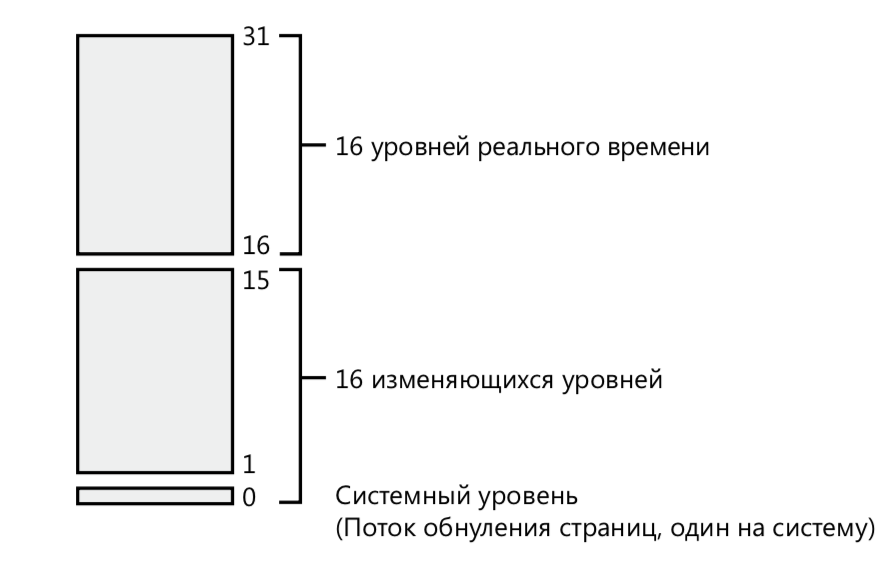
\includegraphics[scale=0.6]{pics/Wind_priority.png}
		
			Рис 2.1: Уровни приоритета потоков в Windows
\end{center}

Уровни приоритета потоков назначаются Windows API и ядром Windows. 

При создании процесса ему присваивается базовый приоритет (по классу которого Windows API систематизирует процессы):
\begin{itemize}
\item реального времени — Real-time (4);
\item высокий — High (3);
\item выше обычного — Above Normal (7);
\item обычный — Normal (2);
\item ниже обычного — Below Normal (5);
\item простоя — Idle (1).
\end{itemize}

После того как  Windows API систематизирует процессы по классу приоритета, присвоенного им при создании, отдельным потокам внутри процесса назначается относительный приоритет:
\begin{itemize}
\item критичный по времени — Time-critical (15);  
\item наивысший — Highest (2);
\item выше обычного — Above-normal (1);
\item обычный — Normal (0);
\item ниже обычного — Below-normal (–1);
\item самый низший — Lowest (–2);
\item простоя — Idle (–15).
\end{itemize}
Числа в списке выше представляют собой приращение, применяемое к базовому приоритету процесса.

Таким образом, в Windows API каждый поток имеет базовый приоритет, являющийся функцией класса приоритета процесса и его относительного приоритета процесса.

Отображение базовых приоритетов процессов на относительные приоритеты отдельных потоков внутри этих процессов приведено на рис. 2.2, где \textit{насыщение} - это уровень, критичный по времени, и уровень простоя.

\begin{center}
		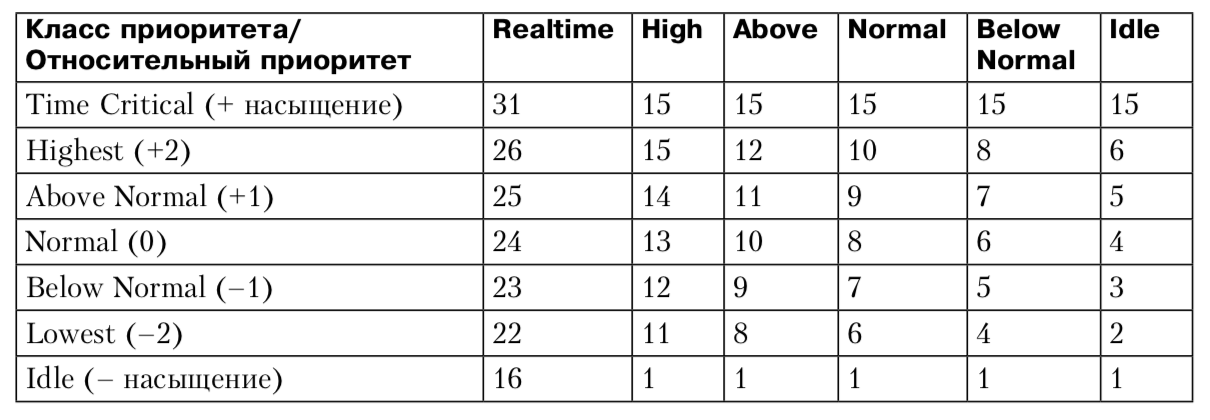
\includegraphics[scale=0.6]{pics/table_Wind_priority.png}
		
			Рис 2.2: Отображение приоритетов ядра Windows на Windows API
\end{center}

Текущий приоритет потока (в динамическом диапазоне от 1 до 15) может быть повышен по причинам, приведенным ниже.
\begin{enumerate}
\item Событие планировщика или диспетчера.
\item Повышение приоритета владельца блокировки.
\item Завершение ввода/вывода (рис. 2.3).
\item Ввода из пользовательского интерфейса.
\item Длительное ожидание ресурса исполняющей системы.
\item Ожидания объекта ядра.
\item Готовый к выполнению поток не был запущен в течение длительного времени.
\item Повышение приоритета проигрывания мультимедиа службой планировщика MMCSS.
\end{enumerate}

\begin{center}
		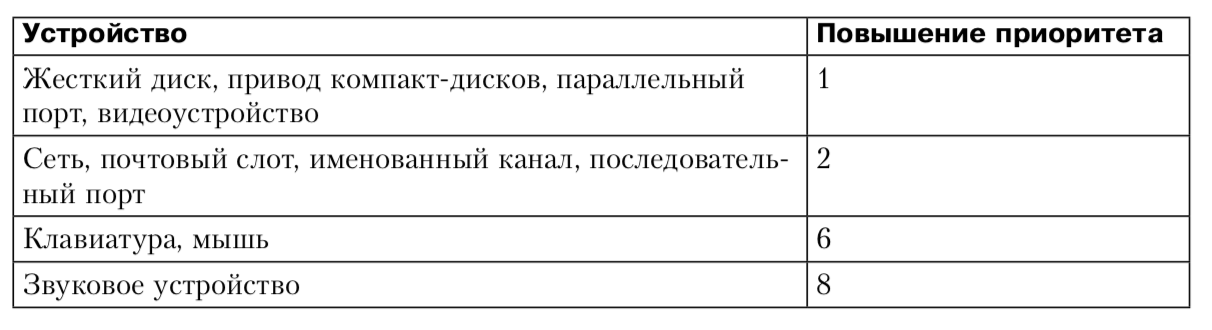
\includegraphics[scale=0.6]{pics/Recommend_InOut.png}
		
			Рис 2.3: Рекомендуемые значения повышения приоритета
\end{center}

Текущий приоритет потока в динамическом диапазоне может быть понижен до базового приоритета путем вычитания всех повышений.

Мультимедийные потоки должны выполняться с минимальными задержками. Эта задача решена в Windows путем повышения приоритетов мультимедийных потоков драйвером MultiMedia Class Scheduler Service (\textbf{MMCSS}). Приложения, реализующие воспроизведение мультимедийного контента, указывают драйверу MMCSS такие задачи, как:
\begin{itemize}
\item аудио;
\item захват;
\item распределение;
\item игры;
\item проигрывание;
\item аудио профессионального качества;
\item задачи администратора многооконного режима.
\end{itemize}

Одно из наиболее важных свойств для планирования потоков называется категорией планирования — Scheduling Category, которое является первичным фактором, определяющим приоритет потоков, зарегистрированных с MMCSS. На рис. 2.4 представлены различные категории планирования.

\begin{center}
		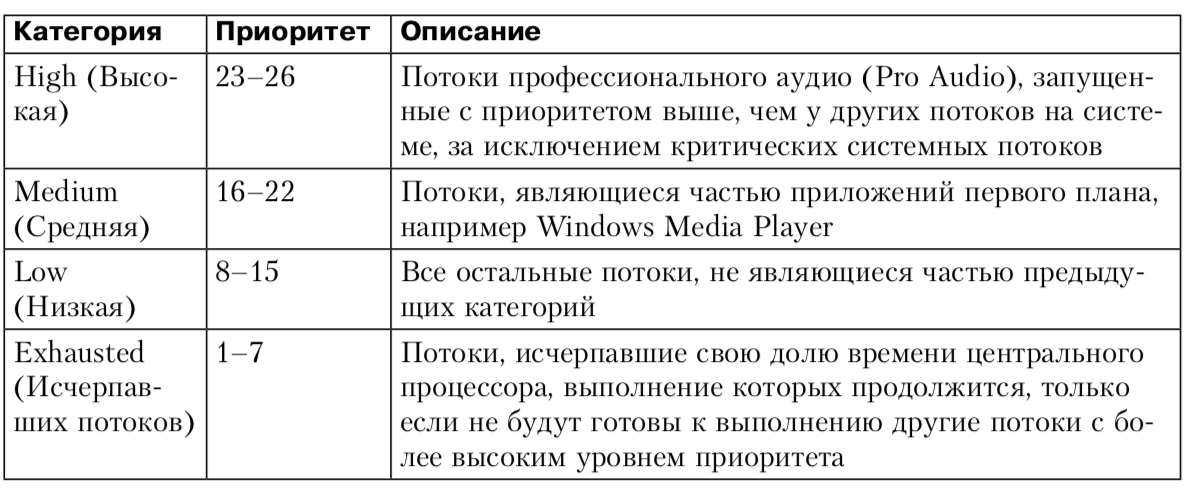
\includegraphics[scale=0.6]{pics/MMCSS.png}
		
			Рис 2.4: Рекомендуемые значения повышения приоритета
\end{center}

Механизм, положенный в основу MMCSS, повышает приоритет потоков внутри зарегистрированного процесса до уровня, соответствующего их категории планирования и относительного приоритета внутри этой категории на гарантированный срок. Затем он снижает категорию этих потоков до Exhausted, чтобы другие, не относящиеся к мультимедийным приложениям потоки, также получили шанс на выполнение.

\section{Пересчет динамических приоритетов для ОС семейства Unix/Linux}

Ядро современных ОС семейства Unix/Linux является вытесняющим для поддержки процессов реального времени, таких как аудио и видео. Это означает, что процесс в режиме ядра может быть вытеснен более приоритетным процессом в режиме ядра.

Очередь готовых к выполнению процессов формируется согласно приоритетам процессов и принципу вытесняющего циклического планирования: процессы с одинаковыми приоритетами выполняются в течении кванта времени циклически друг за другом. Если процесс, имеющий более высокий приоритет, поступает в очередь готовых к выполнению, планировщик вытесняет текущий процесс и предоставляет ресурс более приоритетному.

Приоритет представляет собой целое число из диапазона от 0 до 127. Чем меньше число, тем выше приоритет. В диапазоне \textit{0-49} находятся приоритеты ядра, являющиеся фиксированными величинами. В диапазоне \textit{50-127} – приоритеты прикладных задач, которые могут изменяться во времени в зависимости от факторов, описанных ниже.
\begin{enumerate}
\item Фактор любезности - целое число в диапазоне от 0 до 39 со значением 20 по умолчанию. Чем меньше значение фактора любезности, тем выше приоритет процесса. Фактор любезности процесса может быть изменен суперпользователем с помощью системного вызова nice.
\item Величина использования процессора, измеренная в момент последнего обслуживания им процесса.
\end{enumerate}

Поля структуры \textit{proc}, относящиеся к приоритетам, представлены на рис. 2.5.

\begin{center}
		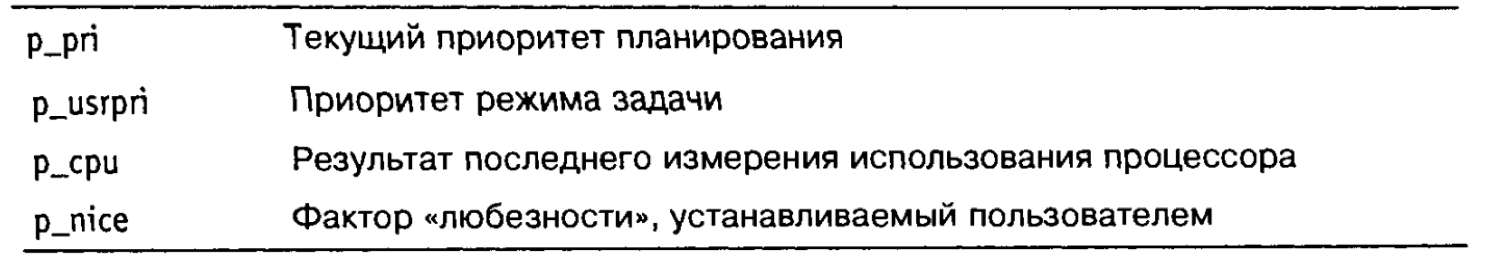
\includegraphics[scale=0.6]{pics/Proc.png}
		
			Рис 2.5: Структура proc
\end{center}

Когда процесс находится в режиме задачи, значения p\_pri и p\_usrpri равны. При пробуждении после блокирования в системном вызове значение текущего приоритета p\_pri  будет повышено для выполнения процесса в режиме ядра. Тогда планировщик использует p\_usrpri для хранения приоритета, который будет назначен при возврате в режим задачи, а p\_pri - для хранения временного приоритета для выполнения в режиме ядра.

Ядро системы связывает приоритет сна с событием или ожидаемым ресурсом, из-за которого процесс может блокироваться. Приоритет сна - это число в диапазоне от 0 до 49, так как он является величиной, определяемой для ядра. Когда процесс просыпается после блокирования в системном вызове, ядро устанавливает в поле p\_pri приоритет сна события или ресурса. Значения приоритета сна в зависимости от события в системе 4.3BSD продемонстрированы на рис. 2.6.

\begin{center}
		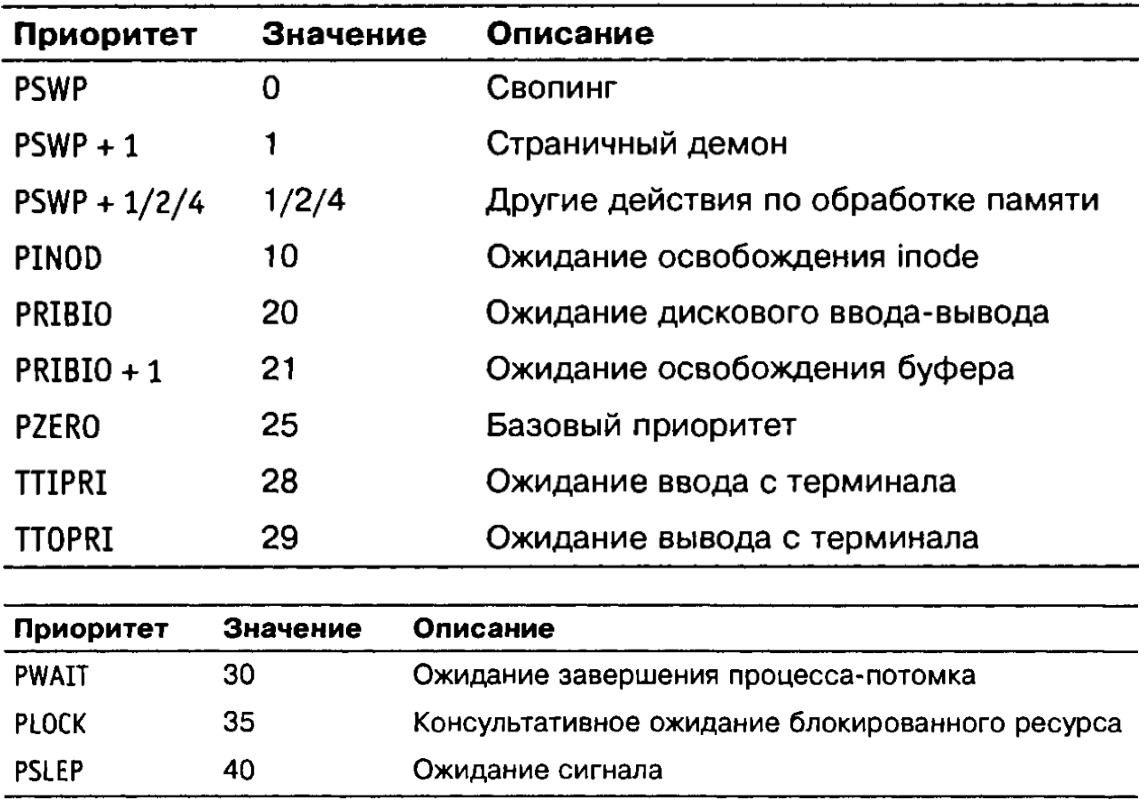
\includegraphics[scale=0.6]{pics/SystemPriority.png}
		
			Рис 2.6: Приоритеты сна в системе 4.3BSD
\end{center}

Поле \textit{p\_cpu} структуры proc, инициализируемое нулем при создании процесса, содержит величину результата последнего сделанного измерения использования процессора процессом. На каждом тике p\_cpu инкрементируется обработчиком таймера на единицу для текущего процесса до максимального значения (127). 
Процедуру schedcpu(), вызываемая ядром каждую секунду, уменьшает значение p\_cpu каждого процесса в зависимости от \textit{фактора "полураспада"} (decay factor). В системе 4.3 BSD значение этого фактора не фиксировано, и для его расчета применяется формула 2.1.

\begin{equation}
decay = (2 * load\_average) / (2 * load\_average + 1)
\end{equation}
где load\_average - это среднее количество процессов, находящихся в состоянии готовности к выполнению, за последнюю секунду. Процедура schedcpu() также пересчитывает приоритеты для режима задачи всех процессов по формуле 2.2.
\begin{equation}
p\_usrpri = PUSER + (p\_cpu / 4) + (2 * p\_nice)
\end{equation}
где PUSER - это базовый приоритет в режиме задачи, равный 50.

Очевидно, что чем больше процессорного времени использовал процесс, тем больше будет его p\_cpu, а, следовательно, и p\_usrpri, что приведет к снижению приоритета. С другой стороны, чем дольше процесс находится в очереди на выполнение, тем меньше будет его p\_cpu благодаря фактору полураспада, и его приоритет будет повышаться. Такая схема позволяет предотвратить зависание низкоприоритетных процессов по вине ОС.

\chapter{Вывод}

Среди функций обработчика прерывания от системного таймера в защищенном режиме в ОС семейств Unix/Linux и Windows можно выделить следующие пункты, являющиеся общими для обоих семейств:
\begin{itemize}
\item инициализирует отложенные действия, относящиеся к работе планировщика (например, пересчет приоритетов);
\item декрементирует счетчики времени (например: часы, счетчик времени отложенных действий);
\item декрементирует квант процессорного времени.
\end{itemize}

Как ОС семейства Unix/Linux, так и ОС семейства Windows являются системами разделения времени с вытеснением и динамическими приоритетами, пересчет которых осуществляется следующим обрзаом:
\begin{itemize}
\item в Windows при создании процесса ему назначается базовый приоритет. Потокам процесса назначается относительный приоритет относительно базового приоритета процесса. Приоритет потока пользовательского процесса может быть пересчитан динамически. 
\item в Unix/Linux приоритет процесса описывается текущим приоритетом и приоритетом процесса в режиме задачи. Приоритет процесса в режиме задачи может быть динамически пересчитан исходя из фактора любезности и величины использования процессора. Приоритеты ядра, наоборот, являются фиксированными величинами.
\end{itemize}

\end{document}